\documentclass{article}
\usepackage[utf8]{inputenc}
\usepackage{biblatex}
\usepackage{relsize}
\addbibresource{bibliography.bib} %Imports bibliography file
\usepackage{hyperref}
\usepackage{listings}
\usepackage{ulem}
\usepackage{float}
\usepackage{graphicx}

\title{Second draft: Benchmarking the Tock operating system for embedded platforms \\[0.2em]\smaller{} CSE 221 Project}
\author{Maximilian Apodaca, Grant Jiang, Gabriel Marcano}
\date{\today}

\begin{document}

\maketitle

\section{Introduction}

%Goals of the project
The goal of this project is to measure CPU and memory operations of the Tock operating system \cite{levy17multiprogramming}. The Tock operating system is undergoing a system call interface change in the near future, so it would be beneficial to benchmark the operating system before the change to form a baseline to compare the changes against. This project will provide that baseline. %https://discord.com/channels/796448392842706954/796448392842706958/801877146548043806

%State the language you used to implement your measurements, and the compiler version and optimization settings you used to compile your code.
Tock is implemented in Rust and supports userland applications written Rust and C/C++. The benchmarks for this project will be written in C/C++ and Rust (FIXME will we do all? Or just a select few). The generated binaries will be compared to ensure that the critical parts of the benchmarks are similar enough in the implementations using different languages (FIXME would time be better spent elsewhere?). %need to see if there's a difference

The following compilers and flags are used for building the benchmarks:
\begin{itemize}
    \item TBD
\end{itemize}

%If you are measuring in an unusual environment (e.g., virtual machine), discuss the implications of the environment on the measurement task (e.g., additional variance that is difficult for you to control for).
%Did you say we can get the cycle count instead?
Benchmark application development will take place on Linux x86\_64 platforms, leveraging QEMU to simulate the OpenTitan platform, and the final results will be acquired by running the benchmarks on an OpenTitan Earl Grey microcontroller instantiation on a Nexys Video Artix-7 FPGA development board \cite{opentitangithub}. Running the tests on the FPGA instead of on QEMU should reduce uncertainty introduced in timing due to QEMU running as a userspace application (and subject to the sharing of systems resources and time). %Currently, accessing the cache is the same time as memory due to single cycle CPU. Maybe later it'll matter.

%who performed which experiments Gabe's email: As far as I am aware, there isn't any networking support, or graphics, but it appears the board does support some IO peripherals, including some AES hardware, some flash memory, and possibly USB as well (I'm not sure yet exactly what drivers the OS has for USB, but the softcore does support USB).
(FIXME We have yet to divide up who performs what experiment, as there is only one board which Gabe has.)

Currently:
Max:
* Measurement Overhead
* Context switch time
Grant:
* Loop Overhead
Gabe:
* Procedure call overhead
* System call overhead
%something about sd card and drivers... lbench hbench...

%Estimate the amount of time you spent on this project.
This project lasts for the duration of the quarter (10 weeks). Each team member plans to spend at most 10 hours per week.

\section{Machine Description}

\subsection{Hardware}
Table \ref{table:1} summarizes the basic specifications of the OpenTitan Earl Grey microcontroller.

\begin{table}[H]
\centering
    \begin{tabular}{|c|c|}
        \hline
        \multicolumn{2}{|c|}{OpenTitan Earl Grey Microcontroller} \\
        \hline
        \hline
        CPU & Ibtex RISC-V RV32IMC \\
        \hline
        External Clock & 100 MHz \\
        \hline
        Instruction cache & 4 kB \\
        \hline
        Data cache & None \\
        \hline
        Pipeline & 2-stage, variable execution length \\
        \hline
        Branch prediction & None (no penalty for not taken) \\
        \hline
        Memory protection & RISC-V Physical Memory Protection\cite{riscv-priv} \\
        \hline
        Memory regions supported & 16 \\
        \hline
        Memory & SRAM, flash, ROM \\
        \hline
        ROM size & 16 kB \\
        \hline
        SRAM size & 64 kB \\
        \hline
        Flash size & 512 kB \\
        \hline
        Interfaces & GPIO, SPI, UART, and JTAG \\
        \hline
        Networking & None \\
        \hline
    \end{tabular}
\caption{OpenTitan Earl Grey Microcontroller specifications}
\label{table:1}
\end{table}

The FPGA bitstream loaded onto the Nexys Video development board implements an OpenTitan Earl Grey microcontroller (\url{https://docs.opentitan.org/hw/top_earlgrey/doc/}). The CPU of the microcontroller is an Ibex RISC-V 32-bit CPU (implementing the RISC-V RV32IMC specification), configured to run at 100 MHz, with 4 kB of instruction cache and no data cache. It has a two stage pipeline consisting of a an Instruction Fetch (IF) stage followed by an Instruction Decode and Execute (ID/EX) stage (some instructions may spend more than one cycle in the execute stage). As configured for the Earl Grey microcontroller, there is no branch prediction (there is no branch penalty if the branch is not taken). The CPU does not support virtual memory, instead implementing Physical Memory Protection (PMP) per the RISC-V Privileged Specification, version 1.11 \cite{riscv-priv}. The CPU PMP is configured to support up to 16 memory protection regions. (for more information on stalls, see \url{https://github.com/lowRISC/ibex/blob/master/doc/03\_reference/pipeline\_details.rst}). There is no floating point unit attached to this CPU.

All of the memory used by the system is kept within the microcontroller; it does not support interfacing with external memory. The microcontroller has 16 kB of ROM used to store the primary boot loader, 512kB of embedded flash (e-flash) to store the actual program data (such as the operating system and application programs and data), and 64 kB of SRAM as scratch space. It takes two cycles to access data from SRAM, and currently also two cycle to read from ROM and e-flash (FIXME confirm this, I know flash is emulated, and that for a long time they had cache disabled, probably because of single cycle memory access timing). ROM, e-flash, and SRAM are mapped to the processors address space and can be accessed directly by the CPU.

The Earl Grey microcontroller supports GPIO, SPI, UART, and JTAG interfaces to interface with it. Internally, it uses a customized data bus to connect all internal peripherals to the CPU (TLUL bus interconnect). (FIXME what is the bandwidth of the different components?)

\subsection{Operating system}

The operating system Tock is an "embedded operating system designed for running multiple concurrent, mutually distrustful applications on Cortex-M and RISC-V based embedded platforms" \cite{tockgithub}. The majority of the operating system is written in Rust, with most parts of the kernel, including all drivers (called capsules), written in safe Rust, and only low level portions hardware specific components written in unsafe Rust and small amounts of assembly language. The kernel uses the Ibex PMP provided by the Earl Grey microcontroller to segregate running userland applications from each other. Figure \ref{figure:1} show the general architecture of Tock.

\begin{figure}[htp]
    \centering
    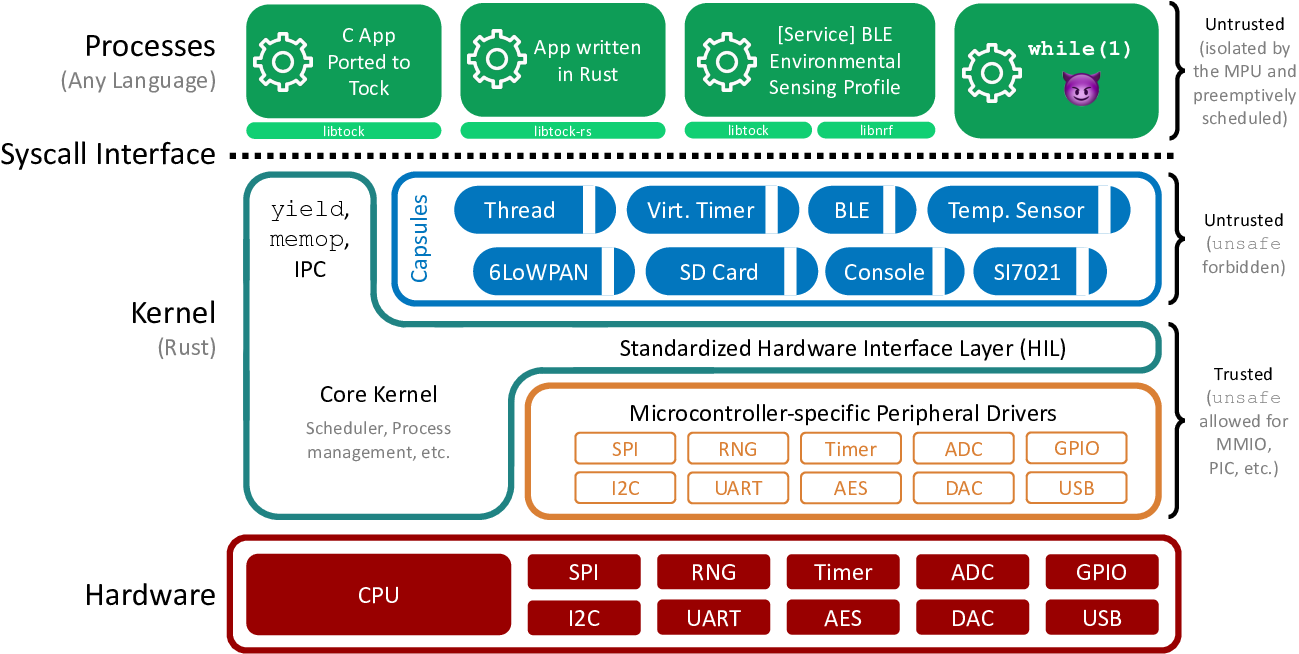
\includegraphics[width=\textwidth]{tock-stack.png}
    \caption{Tock architecture\cite{tockgithub-arch}}
    \label{figure:1}
\end{figure}

The operating system loads applications from e-flash on boot, and there is no way currently to load new applications dynamically the initial loading of applications. Applications run preemptively, while kernel level instructions (capsules/drivers and underlying kernel code) execute cooperatively.

\subsection{Versions and builds}

The version of Tock used for this project supports the original version of the system call interface to the Tock operating system. (FIXME need to determine what commit of Tock to use).

Testing on the Tock operating system git commit X, and on OpenTitan git commit 99cb19827 (built using Xilinx Vivado 2020.1), as this is the latest version currently supported by the Tock operating system.

The operating system was built using the following compiler and linker:
\begin{itemize}
    \item TBD, some kind of LLVM 11 or 12 and a modern enough clang
\end{itemize}

% Measurement overhead: Report the overhead of reading time, and report the overhead of using a loop to measure many iterations of an operation.
\section{Operations and Methodology}

The operations benchmarked for this project are grouped in the following categories:

\begin{itemize}
    \item CPU, scheduling, and OS services
    \item Context switching
    \item Memory access
    \item Inter-process communication
    \item Disk access
\end{itemize}

There is no networking support in the Earl Grey microcontroller.

This section contains the methodologies and results for each of these categories. Benchmarking methods are inspired by the approaches taken by lmbench \cite{lmbench} and hbench \cite{hbench}.

%The goal of an embedded operating system is to keep overhead low as embedded systems tend to run on slower hardware. For example, a modern AMD CPU (https://www.eembc.org/viewer/?benchmark\_seq=13194) is around 60 times faster per MHz than the Earl Grey microcontroller \cite{earlgrey-docs} CPU used for this project. Overhead was computed by running a series of micro-benchmarks to measure common operations. 

\subsection{CPU, scheduling, and OS services}

libtock-c and libtock-rs provide the runtime interface to the OS for applications. 

%Measurement overhead: Report the overhead of reading time, and report the overhead of using a loop to measure many iterations of an operation.
\subsubsection{Time measurement overhead} \label{subsubsec:time-measurement}

RISC-V offers performance counters, including a cycle counter. The cycle counter is a 64 bit register containing the number of cycles elapsed from an arbitrary starting point. As the Earl Grey CPU core does not have 64 bit general purpose registers, it offers two pseudoinstructions to read the upper and lower halves of the 64 bit counter, $RDCYCLEH$ and $RDCYCLE$ respectively.

The bottom 32 bits of the cycle counter should be sufficient precision to measure all benchmarks in this paper, as no benchmark window should be more than 4 billion cycles. The following is an example of taking a measurement, in assembly in Rust:

%maybe use minted package
\begin{lstlisting}[]
        let timestamp: u32;
        unsafe {
            asm!("RDCYCLE {}", out(reg) timestamp);
        }
    
        // Code to benchmark
    
        let timestamp_end: u32;
        unsafe {
            asm!("RDCYCLE {}", out(reg) timestamp_end);
        }
    
        let cycles = timestamp_end - timestamp;
\end{lstlisting}

And the same code in C/C++:

\begin{lstlisting}[language=c]
        uint32_t timestamp;
        asm ("rdcycle %0" : "=r" (timestamp));
    
        // Code to benchmark
    
        uint32_t timestamp_end;
        asm ("rdcycle %0" : "=r" (timestamp_end));
    
        uint32_t cycles = timestamp_end - timestamp;
\end{lstlisting}

Timing measurement overhead is measured by taking a timestamp before and after a set of timestamp reads. The following C code shows an example:

\begin{lstlisting}[language=c]
        uint32_t timestamp;
        asm ("rdcycle %0" : "=r" (timestamp));
    
        uint32_t timestamp_tmp;
        asm ("rdcycle %0" : "=r" (timestamp_tmp));
        asm ("rdcycle %0" : "=r" (timestamp_tmp));
        
        asm ("rdcycle %0" : "=r" (timestamp_tmp));
        asm ("rdcycle %0" : "=r" (timestamp_tmp));
        
        asm ("rdcycle %0" : "=r" (timestamp_tmp));
        asm ("rdcycle %0" : "=r" (timestamp_tmp));
        
        asm ("rdcycle %0" : "=r" (timestamp_tmp));
        asm ("rdcycle %0" : "=r" (timestamp_tmp));
    
        uint32_t timestamp_end;
        asm ("rdcycle %0" : "=r" (timestamp_end));
    
        uint32_t cycles = (timestamp_end - timestamp)/4;
\end{lstlisting}

The example takes 4 pairs samples back to back, and divides the enclosing timing by the number of pairs sampled to estimate the number of cycles it took for a single sample to execute.

FIXME We should disassemble a test binary to see if procedure calls are optimized out. If not, we should do this test in an assembly language portion.

\subsubsection{Loop overhead}

The CPU pipeline does not use a branch predictor, so there is some overhead for every branch taken (there is no stalls in the pipeline added for a branch that is not taken).
\begin{itemize}
    \item A simple loop
    \item A forcefully alternating loop
    \item More complicated loops (to confirm the presence or absence of a branch predictor)
    \item Large loops to probe for the existence and behavior of the instruction cache
\end{itemize}
    
%Procedure call overhead: Report as a function of number of integer arguments from 0-7. What is the increment overhead of an argument?
\subsubsection{Procedure call overhead}

Per RISC-V calling convention (\url{https://github.com/riscv/riscv-elf-psabi-doc/blob/master/riscv-elf.md}), the only registers that need to be saved by the callee are registers s0-s11 (the stack pointer is unmodified on a procedure call, and does not need to be saved). Arguments are passed in via the a0-a7 registers for integer values (this CPU core does not support floating point instructions). If there are more than eight integer/pointer arguments, the first eight are passed in via registers, and the remainder are passed in via the stack.

FIXME Need to make sure to avoid compiler inlining when benchmarking overhead of procedure call

The methodology for testing is to measure the time between a process call and the first instruction execution in the function, by timestamping before the procedure call, and once again at the start of the procedure in question. The two timestamps are then subtracted, and then the measurement overhead from the \nameref{subsubsec:time-measurement} section is subtracted from the result, providing the time it took for the procedure call to occur. Many different empty procedure calls will be made, with different numbers of arguments, to test the impact of the number of arguments passed on procedure call speed.

%System call overhead: Report the cost of a minimal system call. How does it compare to the cost of a procedure call? Note that some operating systems will cache the results of some system calls (e.g., idempotent system calls like getpid), so only the first call by a process will actually trap into the OS.
\subsubsection{System call overhead} \label{sec:syscalls}

Tock supports four kinds of system calls:
\begin{itemize}
    \item Yield (0) - Yields execution to another process
    \item Subscribe (1) - Used to assign callbacks to respond to system events
    \item Command (2)- Instructs a driver to do something
    \item Allow (3) - Share an area of userspace with the kernel
    \item Memop (4)- Memory manipulation operations
\end{itemize}

System calls can be made through libtock-c and libtock-rs, or by manually calling \texttt{ecall} with the right parameters (\url{https://github.com/tock/tock/blob/master/doc/Syscalls.md#0-yield}).

(FIXME need to test to make sure libtock* functions are optimized properly, so tests don't include procedure call overhead. Worst case scenario, we can do ecall calls manually in C or C++, and/or figure out how to do that in Rust efficiently)

One of the simplest system calls is a Command system call for driver 0, command 2, used to get the current tick count of the alarm driver. The frequency of the alarm driver is given by a system call for driver 0, command 1. See the \nameref{sec:syscalls} section for more information about system calls. libtock-c exposes this system call through the \texttt{alarm\_read()} function, and libtock-rs exposes it through the \texttt{alarm\_read()}.

System call overhead will be tested by acquiring timestamps before and after a series of system calls to get the current alarm tick count. Averaging the measured time over the number of system calls made should produce an estimate of the system call overhead.

% Tock has two ways to cross the kernel-userspace boundary. The first is making a syscall to the kernel, the second is receiving a callback from kernel space. We intend to measure both of these directions. In this experiment we first measured the latency of making a standard syscall by using the memop syscall is it is the most lightweight one. Then we can use a simple capsule to redirect a syscall as a callback to measure the kernel to userspace system call.

FIXME The kernel calling userspace functions in the form of a callback are not really system calls. We can measure the overhead of the kernel calling a userspace function if we really want: "Then we can use a simple capsule to redirect a syscall as a callback to measure the kernel to userspace system call."

\subsubsection{Threading overhead}
%(Does Tock support application level threading? Does it spin up a kernel thread?)

Tock does not support multiple threads per process at the present. What the operating system supports in lieu of threads is the ability to subscribe callbacks to be called in the case of events. (FIXME is there any good way to check the overhead? We can measure how long it takes for a subscribe syscall, but that doesn't actually run the callback-- the callback is run asynchronously. Maybe if there is a way to have the callback run instantly?).

%Task creation time: Report the time to create and run both a process and a kernel thread (kernel threads run at user-level, but they are created and managed by the OS; e.g., pthread_create on modern Linux will create a kernel-managed thread). How do they compare?
\subsubsection{Task creation time}

Tock on the OpenTitan Earl Grey MCU only creates new processes when booting, and there is no way, currently, to create new processes afterwards. Applications are loaded sequentially from e-flash, until all applications are loaded, an invalid application header is found, or the hardware runs out of RAM. After all applications are loaded, the scheduler begins and starts scheduling processes for execution.

(FIXME is there any way to salvage this section? I'm not there is a good way to measure from userland how long it takes to do this. We could modify the kernel for this specific test, but I'd rather not do that, just to keep everything consistent with every other step. Something like this could work, maybe?

We used the debug memory of the FPGA with a modified kernel to measure the process creation time. This was profiled in the same way as the procedure calls.
)

%Context switch time: Report the time to context switch from one process to another, and from one kernel thread to another. How do they compare? In the past students have found using blocking pipes to be useful for forcing context switches. (For insight into why a context switch can be much more expensive than a procedure call, consider the evolution of the Linux kernel trap on x86.) 
\subsubsection{Context Switching}

Tock user-level applications are preempted by the scheduler. Userspace applications can communicate with each other with some IPC facilities provided by the kernel, and this can be used to test context switching by explicitly handing control from one application to another through the Yield system call (FIXME or by having one application Yield from the beginning, and have the other wake it up via IPC, and measure how long it takes for it to wake up). Triggering a context switch by Yield (and or? IPC) and writing the timing counters before and after in each of the processes provides the context switch time. 


% Time can be reported with the $RDCYCLE$, $RDTIME$, and $RDINSTRET$ pseudoinstructions. $RDINSTRET$ measures the number of instructions executed which might be better than the number of cycles or time. %A little more about what benchmark

% Procedure call overhead: Report as a function of number of integer arguments from 0-7. What is the increment overhead of an argument?
% There is only one type of procedure call that works the same for user-space and capsule applications. As a result we can only measure one.
% Additionally we should probably profile the IPC for userland.

% System call overhead: Report the cost of a minimal system call. How does it compare to the cost of a procedure call? Note that some operating systems will cache the results of some system calls (e.g., idempotent system calls like getpid), so only the first call by a process will actually trap into the OS.
% $memop$ syscall is provided by the kernel and not a capsule and as a result could give different performance than a capsule syscall. All other syscalls should have similar overhead. Interestingly we can register callbacks from drivers which we will also need to profile.

% Task creation time: Report the time to create and run both a process and a kernel thread (kernel threads run at user-level, but they are created and managed by the OS; e.g., pthread_create on modern Linux will create a kernel-managed thread). How do they compare?
% Bootloader defines the existing processes, there is no kernel level support for dynamic process creation.

% Context switch time: Report the time to context switch from one process to another, and from one kernel thread to another. How do they compare? In the past students have found using blocking pipes to be useful for forcing context switches. (For insight into why a context switch can be much more expensive than a procedure call, consider the evolution of the Linux kernel trap on x86.) 
% This can be easily triggered with the yield() syscall or we can measure the time between interrupts. Kernel context switches appear to be handled by procedure calls while userland to kernel switches are handled via interrupts. TODO: How do capsules call userland code? Only user-capsule transition.

\subsection{Memory}

The OpenTitan Earl Grey microcontroller has three distinct regions of memory: SRAM, Flash, and ROM, all mapped to the CPU address space.

\subsubsection{RAM access time}
% RAM access time: Report latency for individual integer accesses to main memory and the L1 and L2 caches. Present results as a graph with the x-axis as the log of the size of the memory region accessed, and the y-axis as the average latency. Note that the lmbench paper is a good reference for this experiment. In terms of the lmbench paper, measure the "back-to-back-load" latency and report your results in a graph similar to Fig. 1 in the paper. You should not need to use information about the machine or the size of the L1, L2, etc., caches when implementing the experiment; the experiment will reveal these sizes. In your graph, label the places that indicate the different hardware regimes (L1 to L2 transition, etc.).

%[Toshiba94] quotes 110ns as the random read or write cycle time and this time is more representative of the cycle time.
%The ‘‘vacuum’’ means that there is no other activity on the system bus, including no other loads. While this number is frequently used as the memory latency, it is not very useful. It is basically a ‘‘not to exceed’’ number important only for marketing rea- sons.
%When pressed, however, most will admit that cache misses occur in bursts, resulting in perceived latencies of at least the load-in-a-vacuum latency.

%why use and what is backtoback.
%To test the existence of cache?
%we will use back-to-back load latency as described by the lmbench paper. This test attempts to abuse?
%what if it doesn't implement critical word first?
RAM access time is measured by employing the strategy outlined in the lmbench paper for measuring back-to-back-load latency \cite{lmbench}. The lmbench paper measures back-to-back-load "because it is the only measurement that may be easily measured from software and because we feel that it is what most software developers consider to be memory latency." \cite{lmbench} 

The lmbench paper provides this code fragment as an example of how to measure back-to-back-load latency:
\begin{lstlisting}[language=c]
        p = head;
        while (p->p_next)
            p = p->p_next;
\end{lstlisting}

%The tests will access memory with 16, 32, and 64 bytes in between.

Specifically, the code causes back-to-back-loads if each successive access forces a cache miss. Per the paper, some CPUs implement a ``critical word first" optimization where the ``subblock of the cache line that contains the word being loaded is delivered to the processor before the entire cache line has been brought into the cache." \cite{lmbench} If another load is done, with a resulting cache miss, before the previous cache line is completely loaded the cache the CPU must stall the load until that operation completes. The total time between these loads is the back-to-back-load latency. In order to test back-to-back-load latency, then, each access must be approximately the length of the cache line apart.

The specific approach being taken for this benchmark makes no assumption about the cache size of the Earl Grey CPU, with the goal to demonstrate that there is, in fact, there is no data cache. As such, multiple tests are carried out with data 16, 32, and 64 bytes apart, to show that the behavior does not change regardless of the spacing between data in memory, as expected due to the lack of a data cache.

There is no data cache in the processor so a constant access time should be reported. As there is no data cache, each load and store instruction should complete in a constant number of cycles, ideally one cycle for SRAM, and possibly one cycle for flash as well (based on the implementation of ``flash" in the FPGA bitstream).

%For reference:

% //fill node with junk
% // Goal: each node must be 16/32/64 bytes away from each other, to test for different cache sizes
% // Store cycle count start
% // while looooooooop
% // p->p_next - p > cache line size. maybe use char array
% // Store cycle count end

\subsubsection{RAM bandwidth}
% RAM bandwidth: Report bandwidth for both reading and writing. Use loop unrolling to get more accurate results, and keep in mind the effects of cache line prefetching (e.g., see the lmbench paper).
Memory bandwidth is measured in three approaches, as described by the lmbench paper \cite{lmbench}. The first approach measures copy bandwidth (a combination of read and write bandwidth) by using an existing memory copying routine, in this case memcpy, to copy large buffers from one portion of memory to another. The second approach measures read bandwidth by using a manually unrolled loop to read large amounts of data, printing the sum of all values read (to prevent the compiler from optimizing out the memory accesses). The third approach measures write bandwidth, by writing a constant value over a large memory buffer with the use of an unrolled loop.

The OpenTitan Earl Grey microcontroller has three distinct regions of memory, but only two of these are accessible from userspace in Tock, namely, flash and SRAM. Measurements will be taken from both regions separately.

If SRAM and flash read and writes take two cycle per access, optimally, both read and write bandwidths should be close to 200 MB/s, as the CPU clock is 100MHz.

\subsubsection{Kernel memory operations}
% Page fault service time: Report the time for faulting an entire page from disk (mmap is one useful mechanism). Dividing by the size of a page, how does it compare to the latency of accessing a byte from main memory? 
The Tock operating system does not support virtual memory and thus has no concept of page faults \footnote{There is a pending pull request with similar functionality at \url{https://github.com/tock/tock/pull/2424}}. However, it does support some memory-related system calls. The brk and sbrk memop system calls alter the memory layout, specifically the application boundary, of the current application. Benchmarking brk and sbrk should yield timing about adjustments to memory protection regions.

FIXME? We might want to look at the overhead of the $allow$ syscall instead as this is how we can give a capsule access to process memory.

It is estimated that each system call for brk and sbrk will take roughly double the amount of time to get the timer count (\ref{subsubsec:time-measurement}), due to overhead in updating kernel internal structures and the memory protection unit registers.

\subsection{Network}

While Tock does have support for UDP on IPv6, the Earl Grey microcontroller has no networking hardware.
% We don't have a network connection. This might be a good time to profile the inter process communication framework instead. Here we can measure the time it takes to "transmit" and "receive" data from another process.

% \^This is a lie

FIXME We might want to use IPC or we can attempt to profile USB communication.

\subsection{File System}


Tock does not provide any native filesystem support, but it does provide applications access to raw flash memory.

\subsubsection{Size of file cache}
% Size of file cache: Note that the file cache size is determined by the OS and will be sensitive to other load on the machine; for an application accessing lots of file system data, an OS will use a notable fraction of main memory (GBs) for the file system cache. Report results as a graph whose x-axis is the size of the file being accessed and the y-axis is the average read I/O time. Do not use a system call or utility program to determine this metric except to sanity check.
Tock does not have a file system cache. Instead we might want to profile the instruction cache as reading instructions from disk is by far the most common use. It is possible to write to flash for a program however it is a byte addressable array and has no FS to speak of.

FIXME can we access a filesystem on USB?

\subsubsection{File read time}
% File read time: Report for both sequential and random access as a function of file size. Discuss the sense in which your "sequential" access might not be sequential. Ensure that you are not measuring cached data (e.g., use the raw device interface which bypasses the file system (see "man lsblk" if you are using Linux). Report as a graph with a log/log plot with the x-axis the size of the file and y-axis the average per-block time.
The instruction cache could affect this as flash bandwidth is shared. It would be interesting to measure the read time. We can do this and it should give clean results. We don't have to worry about any caches as our program reads directly from the device.

\subsubsection{Remote file read time}
% Remote file read time: Repeat the previous experiment for a remote file system. What is the "network penalty" of accessing files over the network? You can either configure your second machine to provide remote file access, or you can perform the experiment on a department machine (e.g., APE lab). On these machines your home directory is mounted over NFS, so accessing a file under your home directory will be a remote file access (although, again, keep in mind file caching effects).
We could set up an IPC channel that writes to flash in another process, however there is no support for a TCP stack or file system.

% Contention: Report the average time to read one file system block of data as a function of the number of processes simultaneously performing the same operation on different files on the same disk (and not in the file buffer cache).
\subsubsection{Contention}
We can do this for userspace applications however capsules use a cooperative multiprocessing environment and might give interesting results. We would expect throughput to be slightly less than 1/N * memory bandwidth for each process. 

\section{Measurements and discussion}

\section{Conclusion}

\printbibliography

\end{document}
